\documentclass[a4paper]{article}
\usepackage[utf8]{inputenc}
\usepackage{blindtext}
\usepackage[russian]{babel}
\usepackage[14pt]{extsizes} % для того чтобы задать нестандартный 14-ый размер шрифта
\usepackage{setspace,amsmath}
\usepackage{mhchem} % для химических формул
\thispagestyle{empty}
\graphicspath{ {images/} }

\begin{document}
% НАЧАЛО ТИТУЛЬНОГО ЛИСТА
\begin{center}
%\hfill \break
\large{«Московский физико-технический институт (государственный университет)»}\\
\footnotesize{федеральное государственное автономное образовательное учреждение}\\ 
\footnotesize{высшего образования}\\
 \hfill \break
%\normalsize{Кафедра теории функций и  геометрии}\\
\hfill\break
\hfill \break
\hfill \break
\hfill \break
\large{О природе чёточной молнии}\\
\hfill \break
\hfill \break
\hfill \break
\hfill \break
\large{Ю.Р. Аланакян, Д.А. Буланкин, В.Г. Певгов, Л.В. Смирнов, А.А. Цветков}\\
\hfill \break
\hfill \break
\hfill \break
\hfill \break
\hfill \break
\normalsize{Июль 2018} 
\end{center}
% КОНЕЦ ТИТУЛЬНОГО ЛИСТА

\newpage

\section{Экспериментальная установка}
Устройство, на котором изучались процессы образования плазмоидов, реализовано на основе цилиндрического плазмохимического реактора подобного устройству, описанному в патенте RU 2448768. В реакторе (рис.1) формирование потока происходит в вихревой цилиндрической камере, согласованной с цилиндрической газоразрядной камерой, в которой зажигается тлеющий газовый разряд через пленку проводящей жидкости.
\begin{figure}[h]
    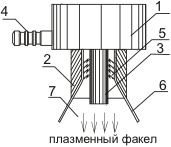
\includegraphics{ShemaUstanovki.png}
    \centering
    \caption{Схема установки}
\end{figure}

В схеме плазмохимического реактора, представленной на Фиг.1, позиции пронумерованы следующим образом:
\begin{enumerate}
    \item камера формирования пленочного потока жидкости,
    \item внешний электрод,
    \item центральный электрод,
    \item штуцер ввода воды,
    \item область горения разряда,
    \item пленочный поток воды,
    \item поток рекомбинирующей плазмы.
\end{enumerate}
В одном из вариантов технического исполнения предлагаемое устройство реализовано на основе цилиндрического плазмохимического реактора подобного устройству, описанному в патенте RU 2448768, в котором формирование потока происходит в вихревой цилиндрической камере, согласованной с цилиндрической газоразрядной камерой, в которой зажигается тлеющий газовый разряд через пленку проводящей жидкости. Через пленку диэлектрической жидкости при этом невозможно зажигание устойчивого тлеющего разряда.

Поток воды подает тангенциально в камеру формирования пленочного потока жидкости 1. В камере формирования при этом образуется тороидальный вихрь. Для этой цели камера изготавливается согласно патенту RU 79384. После формирователя пленочного потока вода движется по спирали, покрывая внутреннюю поверхность внешнего цилиндра – внешнего электрода 2. Электрод 3 предназначен для зажигания тлеющего разряда. При этом создаются условия для реализации электрического разряда с высокими вкладами энергии, что описано в патенте RU 2448768.

Обрабатываемая вода подается через входной штуцер – 4. Между внешним 2 и внутренним 3 электродами зажигается  плазма в электроразрядном промежутке 5. Плазма заполняет коаксиальный промежуток между электродами. 

Плазменный факел 7, выходящий из зоны разряда на расстояние до 5 см., позволяет проследить эволюцию плазмоидов во времени. 

\newpage

\begin{figure}[h]
    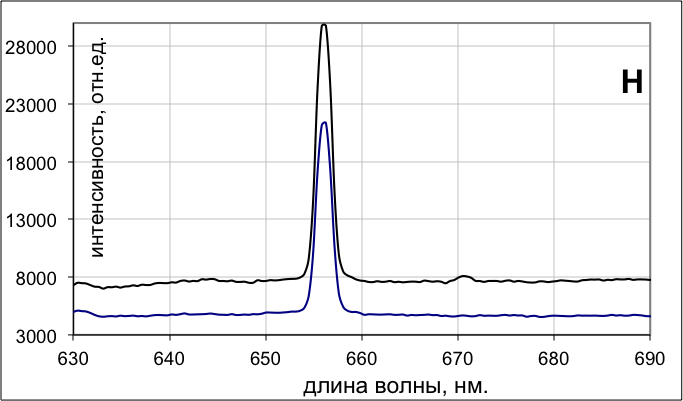
\includegraphics{plot.png}
    \centering
    \caption{Спектр свечения плазменного факела}
\end{figure}

На рис.2 приведен спектр свечения плазменного факела в области основной линии свечения серии Бальмера. Спектры снимались на спектрометре Maya 2000 Pro с использованием ввода сигнала в спектрометр по оптическому волокну, входной конец которого позиционировался вблизи плазменного факела.

\section{Аннотация}

При электрическом разряде в водной среде в атмосферном воздухе образовались светящиеся шары. Иногда шары взрывались. Спектроскопические исследования показали наличие в шаре атомарного водорода. Очевидно, что шары представляют собой диффузно горящий водородный сгусток. Полагаем, что чёточная молния - это такие же диффузно горящие водородные образования.

При электрическом разряде в водной среде неоднократно наблюдали (см., например, [1-3]) следующее явление. В атмосферном воздухе возникали светящиеся объекты шаровидной формы. "Время жизни" этих объектов зависит от радиуса шара и может достигать нескольких секунд. Например, в работе [1], произведя подводный взрыв инициировали удар молнии на водяной фонтан. После разряда молнии в воздухе образовалась цепь светящихся шаров, т. е. возникла чёточная молния. Радиус шара около десяти сантиметров, "время жизни" - одна секунда. В работе [2] указано, что шар, полученный в лаборатории, при столкновении с препятствием взрывается. В результате настоящей работы установлена природа светящегося объекта. Это диффузное горение водорода, содержащегося в шаре. Химическая реакция горения протекает в узком сферическом слое. Кислород поступает сюда из окружающего воздуха диффузионным путем. Теории диффузно горящего шара посвящена работа [6], в которой показано, что в случае, когда в центральной части шара плотность горячего вещества достаточно велика, горящий шар вначале расширяется. Затем устанавливается квазистационарное состояние, при котором поверхность горящего шара движется медленно по сравнению с диффузионными скоростями водорода и кислорода. При механическом воздействии на шар может образоваться гремучая смесь: реакция горения принимает взрывной характер.

Горение водорода - это цепная реакция, брутто-уравнение которой можно записать в виде:
\begin{equation} \label{eq:1}
\ce{H} + \ce{3H2} + \ce{O2} = \ce{3H} + \ce{2H2O} + \ce{2Q},    
\end{equation}
где \(\ce{Q} = 282\cdot10^3\)Дж/моль воды.

Энергия выделяется в основном в процессе рекомбинации \(\ce{H} + \ce{H} = \ce{H2}\). При этом молекулы водорода разлетаются во все стороны от точек поверхности сферы. Таким образом, возникает поток импульса от поверхности горения. Во внутренней области шара давление газа оказывается больше, чем во внешней области. Это способствует сохранению шарообразной формы объекта. 

В статье [6] показано, что в центре шара при квазистационарном горении содержится около 7\% водорода (независимо от радиуса шара). При этом учитывая, что вдали от области горения в воздухе имеется 20\% кислорода и предполагается, что происходит полное сгорание, т. е. концентрация водорода и кислорода на поверхности шара нулевые.

При сближении двух шаров, область между шарами оказывается обедненной кислородом. Это означает, что реакция горения в этой области происходит с меньшей эффективностью. Следовательно, водород проникает в пространство между шарами. В результате объекты сливаются: образуется один шар большого радиуса.

% глава

Теперь обсудим вопрос о том, как происходит разделение водорода и кислорода при электрическом разряде в водной среде.

Разделение тяжелых и легких частиц при электрическом разряде впервые наблюдал Капица [7]. При разряде в аргоновом газе, содержащем примесь дейтерия, он обнаружил, что в области разряда в плазменном шнуре сосредотачиваются только молекулы дейтерия. Теория этого явления изложена в работе [8]. Дело в следующем. Плазменный сгусток, образующийся в области разряда, находится в динамическом равновесии с окружающим газом: поток ионов из плазмы равен потоку нейтральных молекул, влетающих в плазму из окружающей среды. В граничной области плазмы всегда возникает амбиполярное электрическое поле, которое удерживает электроны и ускоряет ионы. Т. е. "следит" за тем, чтобы плазма оставалась "квазинейтральной". Тяжелый молекулы, влетающие в плазму, движутся медленнее, ионизуются в области большого амбиполярного поля и выбрасываются из плазмы. Для процесса "самоочищения" плазмы от тяжелых частиц требуется определенное время. Поэтому при кратковременном (...) разряде этот эффект не наблюдается. Образование сгустков водорода при разряде молнии в водной среде теоретически рассмотрено в работах [9, 10], где показано, что токовый канал молнии неустойчив. Он разбивается на равноудаленные шаровые образования. Экспериментальным подтверждением того, что чёточная молния это диффузно горящие водородные шары могло бы служить обнаружение атомарного водорода при наблюдении чёточной молнии.

Полагаем, что диффузно горящие водородные шары могут образоваться при разряде не только в водной среде, но и в других веществах, содержащих водород. Например, в работе Слюсарева [11] светящиеся объекты в воздухе возникали при электрических разрядах в древесине. Очевидцы опытов Теслы сообщали, что при высокочастотном разряде в катушке возникали светящиеся шарики, разбегающиеся из области разряда.

Заметим, что многие авторы, полученные ими светящиеся объекты, называют шаровыми молниями. Полагаем, что природа рассмотренного нами объекта существенно отличается от природы шаровой молнии.Например, по наблюдениям очевидцев (см., например, [5]) шаровая молния может совершать необычные перемещения и сильно воздействовать на работы электрических приборов. Возможно, шаровая молния это кольцевой вихрь в атмосферном воздухе, который способен автономно перемещаться в пространстве. В вихре сосредоточено самолокализованное высокочастотное электромагнитное поле, под действием которого ионизуется окружающий воздух. Структура такой модели шаровой молнии и возможность её образования обсуждается в работах [12-14]. 

\newpage
\section{Литература}
\begin{enumerate}
    \item G.A. Young NOLTR 61-43 Naval Surface Weapons Center. 1962
    \item П.И. Голубничий, В.М. Громенко, Ю.М. Крутов, Шаровая молния. Сб. тезисов докладов ИВТАН. Москва 1991 стр. 73
    \item А.И. Егоров, С.И. Степанов, Г.Д. Шабалов УФН т.174, с. 107. 2004
    \item И.П. Стаханов. О физической природе шаровой молнии. Научный мир. Москва 1996
    \item Б.М. Смирнов УФН т.116 с.731. 1975
    \item Ю.Р. Аланакян ДАН 415 36, 2007
    \item П.Л. Капица ЖЭТФ 57, 1801, 1969
    \item Ю.Р. Аланакян Письма ЖЭТФ 31, 518, 1980
    \item Ю.Р. Аланакян ДАН 425, 328, 2009
    \item Y.R. Alanakyan Phys. Plasmas 20.082106, 2013
    \item Н.М. Слюсарев. Шаровая молния. Сб. тезисов докладов. ИВТАН Москва 1990
    \item Y.R. Alanakyan Phys. Plasmas 23.054501, 2016
    \item Y.R. Alanakyan Phys. Plasmas 24.044502, 2017
    \item Ю.Р. Аланакян. Шаровая молния - кольцевой вихрь с электромагнитной начинкой. МФТИ. Москва 2017
    
    
\end{enumerate}

 
\end{document}